\documentclass[11pt]{article}

%\usepackage{setspace}
%\documentclass[final,leqno]{siamltex}
\usepackage{smoothing_paper}



\usepackage[section]{placeins}
\usepackage{tabularx,ragged2e,booktabs,caption}
\usepackage{hyperref}

%%%%%%%%%%%%%%%%%%%%%%%%%%%%%%%%chiheb commands

\interfootnotelinepenalty=10000
%%%%%%%%%%%%%%%%%
\newcommand{\ie}{\emph{i.e.}}
\newcommand{\eg}{\emph{e.g.}}
\newcommand{\cf}{\emph{cf.}}
\newcommand{\prob}[1]{\mathrm{P}\left(#1\right)}
\newcommand{\expt}[1]{\mathrm{E}\left[#1\right]}
\newcommand{\expth}[1]{\hat{\mathrm{E}}\left[#1\right]}



\newcommand{\rset}{\mathbb{R}}
\newcommand{\nset}{\mathbb{N}}
\newcommand{\zset}{\mathbb{Z}}



\newcommand{\PERIOD}{.}
\newcommand{\COMMA}{,}
\newcommand{\BIGSPACE}{\,\,\,\,\,\,\,}



\newcommand{\Ordo}[1]{{\mathcal{O}}\left(#1\right)}
\newcommand{\ordo}[1]{{o}\left(#1\right)}

%%%%%%%%%%%%%%%%%%%%%%%%%%%%%%%%%%%%%%%%%%%%%%%%%%%%%%%%%%%%%%%%%%%%%%%%
%%
%% DO WE RELLY NEED THE FOLLOWING??

%%  new margin
%%%%%%%%%%%%%%%%%%%%%%%%%%%%%%%%%%%%%%%%%%%
\pagestyle{plain}                                                      %%
%%%%%%%%%% EXACT 1in MARGINS %%%%%%%                                   %%
\setlength{\textwidth}{6.5in}     %%                                   %%
\setlength{\oddsidemargin}{0in}   %%   
\setlength{\evensidemargin}{0in}  %%        
\setlength{\textheight}{8.5in}    %%       
\setlength{\topmargin}{-0.2in}    %%   
\setlength{\headheight}{0in}      %%    
\setlength{\headsep}{0in}         %%                   
\setlength{\footskip}{.5in}       %%                       
%%%%%%%%%%%%%%%%%%%%%%%%%%%%%%%%%%%%                                   %%
\newcommand{\required}[1]{\section*{\hfil #1\hfil}}                    %%
\renewcommand{\refname}{\hfil References Cited\hfil}                   %%

\def\SMALLSKIP{\smallskip}
\def\MEDSKIP{\medskip}
\def\BIGSKIP{\bigskip}

%%
%%%%%%%%%%%%%%%%%%%%%%%%%%%%%%%%%%%%%%%%%%%%%%%%%%%%%%%%%%%%%%%%%%%%%

\makeatletter
\def\BState{\State\hskip-\ALG@thistlm}
\makeatother



%%%%%%%%%%%%%%%%%%%%%%%%%%%%%%%%%%%%%%%%

\title{Quadrature Error Estimation  for option pricing under the rough Bergomi model} 


%\pagestyle{myheadings}
\thispagestyle{plain}

\setcounter{tocdepth}{1}

\begin{document}





\section{Problem setting}\label{sec:Problem setting}
In this section, we introduce the pricing framework that we are considering in this work. We start  by giving some details for the rBergomi model proposed in \cite{bayer2016pricing}. We then derive the formula of the price of a European call option under the rBergomi model, in Section \ref{sec:Option pricing under rBergomi model}. This section corresponds  to the first stage of our approach, that is the analytical smoothing step. Finally, we explain  some details about the hybrid scheme that we use to simulate the dynamics of asset prices under the rBergomi model.

\subsection{The rBergomi model}\label{sec:The rBergomi model}

We use  the rBergomi model for the price process $S_t$ as defined in  \cite{bayer2016pricing}, normalized to $r=0$, which is defined by

\begin{align}\label{eq:rBergomi_model1}
	dS_t = \sqrt{v_t} S_t dZ_t, \nonumber \\
	v_t = \xi_0(t) \exp\left( \eta \widetilde{W}_t^H - \frac{1}{2} \eta^2 t^{2H} \right),
\end{align}
where the Hurst parameter $0 < H < 1$  and  $\eta>0$. We refer to $v_t$ as the variance process, and $\xi_0(t) = \expt{v_t}$ is  the forward variance curve.  Here, $\widetilde{W}^H $ is a certain Riemann-Liouville fBm
process,  defined by
\begin{align}\label{eq:Volterra process}
	\widetilde{W}_t^H = \int_0^t K^H(t,s) dW_s^1, \quad t \ge 0 \COMMA
\end{align}
where the kernel $K^H : \rset_+ \times \rset_+ \rightarrow \rset_+$ is
\begin{align*}
 \quad K^H(t,s) = \sqrt{2H} (t-s)^{H - 1/2},\quad \forall \: 0 \le s \le t.
\end{align*}

%We note that the map $s \rightarrow K^H(s,t)$ belongs to $L^2$, so
%that the stochastic integral \eqref{eq:Volterra process} is well defined.
 $\widetilde{W}^H $ is a centered, locally $(H-\epsilon)$- H\"older continuous, Gaussian process with $\text{Var}\left[\widetilde{W}^H_t \right] = t^{2H}$, and a dependence structure defined by 
 \begin{equation*}
 \expt{\widetilde{W}^H_u  \widetilde{W}^H_v}=u^{2H} G\left(\frac{v}{u} \right),\quad v >u \COMMA
 \end{equation*}
 where for $x \ge 1$ and $\gamma=\frac{1}{2}-H$
 
  \begin{equation*}
G(x)=2H \int_{0}^1 \frac{ds}{(1-s)^{\gamma} (x-s)^{\gamma}}.
 \end{equation*}
 

$W^1, Z$ denote two \emph{correlated} standard Brownian motions with correlation $\rho \in [-1,1]$, so that we can write
\begin{align*}
	Z:=\rho	W^1+ \bar{\rho}W^\perp = \rho W^1+\sqrt{1-\rho^2} W^\perp,
\end{align*}
where $(W^1,W^\perp)$ are two independent standard Brownian motions.
Therefore, the solution to \eqref{eq:rBergomi_model1}, with $S(0)=S_0$, can be written as 

\begin{align}\label{eq:rBergomi_model}
	S_t&= S_0  \operatorname{exp}\left( \int_{0}^{t} \sqrt{v(s)} dZ(s)- \frac{1}{2} \int_{0}^{t} v(s) ds   \right),\quad S_0>0 \nonumber\\
	v_u&=\xi_0(u) \operatorname{exp}\left( \eta \widetilde{W}_u^H- \frac{\eta^2}{2} u^{2H} \right), \quad \xi_0>0 \PERIOD
\end{align}


The filtration $(\mathcal{F}_t)_{t\ge 0}$ can here be taken as the one generated by the two-dimensional Brownian motion $(W^1,W^\perp)$ under the risk neutral measure $\mathbb{Q}$, resulting in  a filtered probability space $(\Omega,\mathcal{F}, \mathcal{F}_t,\mathbb{Q})$. The stock price process $S$ is clearly then a local
$(\mathcal{F}_t)_{t\ge 0}$-martingale and a supermartingale, therefore integrable.  We shall henceforth use the notation $\expt{.} = E^{\mathbb{Q}}\left[. \mid \mathcal{F}_0\right]$ unless we state otherwise.








\subsection{Option pricing under the rBergomi model}\label{sec:Option pricing under rBergomi model}

We are interested in pricing European call options under the rBergomi model. Assuming $S_0 = 1$, and using the conditioning argument on the $\sigma$-algebra generated by $W^1$ (an argument first used by \cite{romano1997contingent} in the context of Markovian stochastic volatility  models), we can  show that the call price is given by

\begin{align}\label{BS_formula_rbergomi}
	C_{\text{RB}}\left( T, K \right) &= \text{E}\left[ \left(S_T - K \right)^+ \right]  \nonumber\\
	&=\expt{\expt{(S_T-K)^+ \mid \sigma(W^1(t) ,t \le T)}}\nonumber \\
	&=\text{E}\left[C_{\text{BS}}\left( S_0 = \operatorname{exp}\left(\rho \int_0^T \sqrt{v_t} dW_t^1 - \frac{1}{2}
	\rho^2 \int_0^T v_t dt\right),\ k = K, \ \sigma^2 = (1-\rho^2)
	\int_0^T v_t dt \right) \right],
\end{align}
where $C_{\text{BS}}(S_0,k,\sigma^2)$ denotes the Black-Scholes call price, for initial spot price $S_0$, strike price $k$ and volatility $\sigma^2$.

To show \eqref{BS_formula_rbergomi}, we use the orthogonal decomposition of $S_t$ into $S_{t}^1$ and $S_{t}^2$, where

\begin{align*}
	S_t^1:=\mathcal{E}\{ \rho \int_{0}^{t}  \sqrt{v_s} dW_s^1\}, \: S_t^2:= \mathcal{E}\{ \sqrt{1-\rho^2} \int_{0}^{t}  \sqrt{v_s} dW_s^\perp  \}	,
\end{align*}

and $\mathcal{E}(.)$ denotes the stochastic exponential \footnote{For a continuous semimartingale $Z$, the
stochastic exponential is defined as $\mathcal{E}(Z)_t:=\exp\left(Z_t-Z_0- \frac{1}{2} [Z]_t  \right)$.}; then we obtain by conditional log-normality
\begin{align*}
	\log S_t \mid \mathcal{F}_t^1 \sim \mathcal{N}\left( \log S_t^1-\frac{1}{2} (1-\rho^2) \int_{0}^{t} v_s ds , (1-\rho^2) \int_{0}^{t} v_s ds \right),
\end{align*} 

where $\mathcal{F}_t^1= \sigma\{ W_s^1: s\le t\}$. Therefore, we obtain \eqref{BS_formula_rbergomi}.



We point out that the analytical smoothing, based on conditioning, performed in \eqref{BS_formula_rbergomi} enables us to uncover the available regularity, and hence  get a smooth, analytic integrand inside the expectation. Therefore, applying sparse quadrature techniques becomes an adequate option for computing the call price as we will investigate later. A similar conditioning was used in \cite{mccrickerd2017turbocharging} but for variance reduction purposes.

\subsection{Simulation of the rBergomi model}\label{sec:Simulation of the rBergomi model}

One of the numerical challenges encountered in the simulation of the rBergomi dynamics  is the computation of the terms  $\int_{0}^{T} \sqrt{v_t} dW_t^1$ and $V=\int_{0}^{T} v_t dt$ as in \eqref{BS_formula_rbergomi}, mainly because of the singularity of the Volterra kernel $K^H(s,t)$ at the diagonal $s = t$. In fact,  one needs to jointly simulate the two-dimensional Gaussian process $(W_t^1, \widetilde{W}^H_t: 0 \le t \le T)$, resulting in $W^1_{t_1},\dots, W_{t_N}$ and $\widetilde{W}^H_{t_1},\dots, \widetilde{W}^H_{t_N}$ along a given time grid $t_1 <\dots < t_N$. In the literature, there are essentially three possible ways to achieve this:
 \begin{enumerate}
 	\item[i)] \textbf{Simple Euler discretization}: Euler discretization of the integral \eqref{eq:Volterra process}, defining $\widetilde{W}^H$, together with classical simulation of increments of $W^1$. This is inefficient because the integral is singular and adaptivity probably does not help, as the singularity moves with time. For this method, we need an $N$-dimensional random Gaussian input vector to produce one (approximate, inaccurate) sample of $W^1_{t_1},\dots, W^1_{t_N}, \widetilde{W}^H_{t_1},\dots, \widetilde{W}_{t_N}$.
 	
 	\item[ii)] \textbf{Covariance based approach}: Given that $W^1_{t_1},\dots, W^1_{t_N}, \widetilde{W}^H_{t_1},\dots, \widetilde{W}_{t_N}$ together forms a ($2N$)-dimensional Gaussian random vector with computable covariance matrix. One can use Cholesky decomposition of the covariance matrix to produce exact samples of $W^1_{t_1},\dots, W^1_{t_N}, \widetilde{W}^H_{t_1},\dots, \widetilde{W}_{t_N}$, but unlike the first way, we need $2 \times N$-dimensional Gaussian random vector as
 	input. This method is exact but slow (see  \cite{bayer2016pricing} and Section $4$ in \cite{bayer2017short} for more details about this scheme). The simulation  requires $\Ordo{N^2}$ flops. 
 	
 	\item[iii)]  \textbf{The hybrid scheme of \cite{bennedsen2017hybrid}}: This scheme uses a different approach, which is essentially based on  Euler discretization as the first way but crucially improved by moment
 	matching for the singular term in the left point rule. It is also
 	inexact in the sense that samples produced here do not exactly have the distribution of $W^1_{t_1},\dots, W^1_{t_N}, \widetilde{W}^H_{t_1},\dots, \widetilde{W}_{t_N}$, however they are much more accurate then samples produced from method $(i)$, but much faster than method $(ii)$. As in method $(ii)$, in this case, we need a $2 \times N$-dimensional Gaussian random input vector to produce one
 	sample of $W^1_{t_1},\dots, W^1_{t_N}, \widetilde{W}^H_{t_1},\dots, \widetilde{W}_{t_N}$. 
 \end{enumerate}
In this work, we adopt approach  $(iii)$ for the simulation of the rBergomi asset price. As explained in \cite{bennedsen2017hybrid}, the scheme discretize $\widetilde{W}^H$ process into Wiener integrals of power functions and a Riemann sum, appearing from approximating the kernel by power functions near the origin and step functions elsewhere (see \eqref{eq:Hybrid_scheme}). We utilize the first order variant $(\kappa=1) $ of the hybrid scheme, which is based on the following approximation

\begin{equation}\label{eq:Hybrid_scheme}
\widetilde{W}^H_{\frac{i}{N}} \approx \bar{W}^H_{\frac{i}{N}}:= \sqrt{2H} \left(\int_{\frac{i-1}{N}}^{\frac{i}{N}} \left(\frac{i}{N} -s\right)^{H-\frac{1}{2}} dW_u^1+\sum_{k=2}^{i} \left(\frac{b_k}{N}\right)^{H-\frac{1}{2}} \left(W_{\frac{i-(k-1)}{N}}^1-W_{\frac{i-k}{N}}^1\right)\right) \COMMA
\end{equation}
where $N$ is the number of time steps and 
$$ b_k:=\left(\frac{k^{H+\frac{1}{2}}-(k-1)^{H+\frac{1}{2} }}{H+\frac{1}{2}}\right)^{\frac{1}{H-\frac{1}{2}}} \PERIOD$$

The sum in \eqref{eq:Hybrid_scheme} requires the most computational effort in the simulation. Given that \eqref{eq:Hybrid_scheme} can be seen as discrete convolution  (see \cite{bennedsen2017hybrid}), we employ the fast Fourier transform to evaluate it, which results in  $\Ordo{N \log N}$ floating point operations.


We note that the variates $\bar{W}_0^{H},\bar{W}_1^{H},\dots,\bar{W}_{\frac{[Nt]}{N}}^{H}$ are  generated by sampling $[Nt]$ i.i.d draws from a $(\kappa+1)$-dimensional Gaussian distribution and computing a discrete convolution. We denote these pairs  of Gaussian random variables from now on by $(\mathbf{W}^{(1)},\mathbf{W}^{(2)})$.

 
\section{Quantity of interest and error bounds}\label{sec:Quantity of interest and error bounds }
We recall that our goal is to compute the expectation in \eqref{BS_formula_rbergomi}. In fact, as seen in Section \ref{sec:Simulation of the rBergomi model}, we need   $2N$-dimensional Gaussian inputs for the used  hybrid  scheme ($N$ is the number of time steps in  the time grid), namely
\begin{itemize}
	\item $\mathbf{W}^{(1)}=\{W^{(1)}_i\}_{i=1}^N$: The $N$ Gaussian random variables that are defined in Section  \ref{sec:The rBergomi model}.
	\item $\mathbf{W}^{(2)}=\{W^{(2)}_j\}_{j=1}^N$: \red{An artificially} introduced $N$ Gaussian random variables that are used for left-rule points in the hybrid scheme, as explained in Section  \ref{sec:Simulation of the rBergomi model}.
\end{itemize}

We can rewrite \eqref{BS_formula_rbergomi} as 

\red{
\begin{align}\label{BS_formula_rbergomi_2}
C_{\text{RB}}\left( T, K \right)&=\text{E}\left[C_{\text{BS}}\left( S_0 = \operatorname{exp}\left(\rho \int_0^T \sqrt{v_t} dW_t^1 - \frac{1}{2}
\rho^2 \int_0^T v_t dt\right),\ k = K, \ \sigma^2 = (1-\rho^2)
\int_0^T v_t dt \right) \right], \nonumber \\
&\approx \int_{\rset^{2N}} C_{BS} \left(G(\mathbf{W}^{(1)},\mathbf{W}^{(2)})\right) \rho_{N}(\mathbf{W}^{(1)})  \rho_{N}(\mathbf{W}^{(2)}) d\mathbf{W}^{(1)} d\mathbf{W}^{(2)}:=C_{RB}^{N},
\end{align}
}
where $G$  maps  $2N$ independent standard Gaussian random inputs to the parameters fed to Black-Scholes formula, and  $\rho_N$ is the multivariate Gaussian density, given by 

\begin{equation*}\label{eq: multivariate gaussian distribution}
\rho_N(\mathbf{z})=\frac{1}{(2 \pi)^{N/2}} e^{-\frac{1}{2} \mathbf{z}^T \mathbf{z}} \PERIOD
\end{equation*} 

Therefore, the initial integration problem that we are solving lives in $2N$-dimensional space, which becomes very large as the number of time steps $N$, used in the hybrid scheme, increases.


Our approach of approximating the expectation in \eqref{BS_formula_rbergomi_2} is based on MISC, proposed in \cite{haji2016multi}. We describe the  MISC method in our context in Section \ref{sec:Details of the MISC}.  To make an effective use of MISC, we  first apply two transformations to overcome the issue of facing a high dimensional integrand due to the discretization scheme used for simulating the rBergomi dynamics. The first transformation consists of applying a hierarchical  path generation method, based on Brownian
bridge (Bb) construction, with the aim of reducing the effective dimension as  described  in Section \ref{sec:Brwonian bridge construction}. The second transformation consists of applying Richardson extrapolation to reduce the bias, resulting in reducing  the maximum number of dimensions needed for the integration problem. Details about  Richardson extrapolation  are provided in Section \ref{sec:Richardson extrapolation}.




If we denote by $\mathcal{E}_{\text{tot}}$ the total error of approximating the  expectation in \eqref{BS_formula_rbergomi} using the MISC estimator, $Q_N$, then we have a natural error decomposition
\begin{align}\label{eq:total_error}
\mathcal{E}_{\text{tot}} & \le \abs{C_{\text{RB}}-C_{\text{RB}}^N}+\abs{C_{\text{RB}}^N-Q_{N}}\nonumber\\
  & \le \mathcal{E}_B(N)+ \mathcal{E}_Q(\text{TOL}_{\text{MISC}},N),
\end{align}
where  $\mathcal{E}_Q$ is the quadrature error, $\mathcal{E}_B$  is the bias, and $C_{\text{RB}}^N$ is the biased price computed with $N$ time steps as given by \eqref{BS_formula_rbergomi_2}.

\subsection{The MISC method}\label{sec:Details of the MISC}

We assume that we want to approximate the expected value $\text{E}[f(Y)]$ of an analytic function $f\colon \Gamma \to \rset$ using a tensorization of quadrature formulas over $\Gamma$.

To introduce simplified notations, we start with the one-dimensional case. Let us denote by $\beta$ a non negative integer, referred to as a ``stochastic discretization level", and by $m: \nset \rightarrow \nset$  a strictly increasing function with $m(0)=0$ and $m(1)=1$, that we call  ``level-to-nodes function". At level $\beta$, we consider a set of $m(\beta)$ distinct quadrature points in $\rset$, $\mathcal{H}^{m(\beta)}=\{y^1_\beta,y^2_\beta,\dots,y_\beta^{m(\beta)}\} \subset \rset$, and a set of quadrature weights, $\boldsymbol{\omega}^{m(\beta)}=\{\omega^1_\beta,\omega^2_\beta,\dots,\omega_\beta^{m(\beta)}\}$. We also let $C^0(\rset)$ be the set of real-valued continuous functions over $\rset$. We then define the quadrature operator as

\red{
\begin{equation}
Q^{m(\beta)}:C^0(\rset) \rightarrow \rset, \quad Q^{m(\beta)}[f]= \sum_{j=1}^{m(\beta)} f(y^j_\beta) \omega_\beta^j.
\end{equation}

}



In our case, we have in \eqref{BS_formula_rbergomi_2} a multi-variate integration problem with,  $f=C_{\text{BS}}\circ G$, $\mathbf{Y}=(\mathbf{W}^{(1)},\mathbf{W}^{(2)})$, and  $\Gamma=\rset^{2N}$, in the previous notations.  Therefore,  we define for any multi-index $\boldsymbol{\beta} \in \nset^{2N}$

\red{
$$Q^{m(\boldsymbol{\beta})}: \Gamma \rightarrow \rset,\quad  Q^{m(\boldsymbol{\beta})}= \bigotimes_{n = 1}^{2N} Q^{m(\beta_n)} \COMMA $$
}

where the $n$-th quadrature operator is understood to act only on the $n$-th variable of $f$. Practically, we obtain the value of $Q^{m(\boldsymbol{\beta})}[f]$  by using the grid $\mathcal{T}^{m(\boldsymbol{\beta})}= \prod_{n = 1}^{2N}  \mathcal{H}^{m(\beta_n)}$, with cardinality $\#\mathcal{T}^{m(\boldsymbol{\beta})}=\prod_{n=1}^{2N} m (\beta_n)$, and computing

\red{
$$ Q^{m(\boldsymbol{\beta})}[f]= \sum_{j=1}^{\#\mathcal{T}^{m(\boldsymbol{\beta})}} f(\hat{y}_j) \bar{\omega}_j \COMMA$$
}

where $\hat{y}_j \in \mathcal{T}^{m(\boldsymbol{\beta})}$ and $\bar{\omega}_j$ are  products of weights of the univariate quadrature rules. To simplify notation, hereafter, we replace  $Q^{m(\boldsymbol{\beta})}$ by $Q^{\boldsymbol{\beta}}$.

\begin{remark}
We note that the quadrature points are chosen to optimize the convergence properties of the quadrature error.  For instance, in our context, since we are dealing with Gaussian densities, using Gauss-Hermite quadrature points is the appropriate choice.
\end{remark}

A direct approximation $\expt{f[\mathbf{Y}]} \approx Q^{\boldsymbol{\beta}}[f]$ is not an appropriate option  due to the well-known ``curse of dimensionality". We use MISC, which is a hierarchical adaptive sparse grids quadrature strategy that uses  stochastic discretizations  and classic sparsification approach to obtain an effective approximation scheme for $\expt{f}$. 

 For the sake
of concreteness, in our setting, we are left with a $2N$-dimensional Gaussian random input, which is chosen independently, resulting in  $2N$ numerical parameters for MISC, which we use as the basis of the multi-index construction. For a multi-index $\boldsymbol{\beta} = (\beta_n)_{n=1}^{2N} \in \mathbb{N}^{2N}$, we denote  by
$Q_N^{\boldsymbol{\beta}}$,   the result of approximating \eqref{BS_formula_rbergomi_2} with a number of quadrature points  in the $i$-th dimension equal to  $m(\beta_i)$. We further define the set of
differences $\Delta Q_N^{\boldsymbol{\beta}}$ as follows: for a single index $1 \le i \le 2N$,
let




\begin{equation}
\Delta_i Q_N^{\boldsymbol{\beta}} \coloneqq \left\{ 
\aligned 
 Q_N^{\boldsymbol{\beta}} &- Q_N^{\boldsymbol{\beta}'}  \text{, with } \boldsymbol{\beta}' =\boldsymbol{\beta} - e_i, \text{ if } \boldsymbol{\beta}_i>0 \\
 Q_N^{\boldsymbol{\beta}} &, \quad  \text{ otherwise}
\endaligned
\right.
\end{equation}
where $e_i$ denotes the $i$th $2N$-dimensional unit vector. Then, $\Delta
Q_N^{\boldsymbol{\beta}}$ is defined as
\begin{equation}
\Delta Q_N^{\boldsymbol{\beta}} \coloneqq \left( \prod_{i=1}^{2N} \Delta_i \right) Q_N^{\boldsymbol{\beta}}.
\end{equation}
For instance, when $N = 1$, then 
\begin{multline*}
	\Delta Q_1^{\boldsymbol{\beta}} = \Delta_2 \Delta_1 Q_1^{(\beta_1, \beta_2)} = \Delta_2\left( Q_1^{(\beta_1,
		\beta_2)} - Q_1^{(\beta_1-1,\beta_2)} \right) = \Delta_2 Q_1^{(\beta_1,
		\beta_2)} - \Delta_2 Q_1^{(\beta_1-1,\beta_2)} 
	\\= Q_1^{(\beta_1, \beta_2)} - Q_1^{(\beta_1, \beta_2-1)} - Q_1^{(\beta_1-1, \beta_2)} + Q_1^{(\beta_1-1, \beta_2-1)}.
\end{multline*}

\red{Given the definition of $C_{RB}^{N}$ by \eqref{BS_formula_rbergomi_2}, we have the telescoping property
\begin{equation}
C_{RB}^{N}=Q_N^\infty = \sum_{\beta_1=0}^\infty \cdots \sum_{\beta_{2N} = 0}^\infty \Delta
Q_N^{(\beta_1, \ldots, \beta_{2N})} = \sum_{\boldsymbol{\beta} \in \mathbb{N}^{2N}} \Delta Q_N^{\boldsymbol{\beta}}.
\end{equation}
}

 The MISC estimator used for approximating \eqref{BS_formula_rbergomi_2}, and using a set of multi-indices $\mathcal{I}\subset \nset^{2N}$ is given by
\begin{equation*}
	Q_N^{\mathcal{I}} \coloneqq \sum_{\boldsymbol{\beta} \in \mathcal{I}} \Delta Q_N^{\boldsymbol{\beta}}.
\end{equation*}

The quadrature error in this  case  is given by
\begin{equation}\label{eq:quadrature error}
	\mathcal{E}_Q(\text{TOL}_{\text{MISC}},N) =\abs{Q_N^\infty - Q_N^\mathcal{I}} \le \sum_{\boldsymbol{\beta} \in \mathbb{N}^{2N} \setminus
		\mathcal{I}} \abs{\Delta Q_N^{\boldsymbol{\beta}}}.
\end{equation}

\red{
We define the work contribution, $\Delta \mathcal{W}_{\boldsymbol{\beta}}$, to be the computational cost  required to add  $\Delta Q_N^{\boldsymbol{\beta}}$ to $Q^{\mathcal{I}}_N$, and the error contribution, $\Delta E_{\boldsymbol{\beta}}$, to be  a measure of how much the quadrature error, defined in \eqref{eq:quadrature error}, would decrease once $\Delta Q_N^{\boldsymbol{\beta}}$  has been added to  $Q^{\mathcal{I}}_N$, that is 


\begin{align}\label{eq:Work_error_contributions}
\Delta \mathcal{W}_{\boldsymbol{\beta}} &= \text{Work}[Q^{\mathcal{I} \cup \{\boldsymbol{\beta}\}}_N]-\text{Work}[Q^{\mathcal{I}}_N] \nonumber\\
\Delta E_{\boldsymbol{\beta}} &= \abs{Q^{\mathcal{I} \cup \{\boldsymbol{\beta}\}}_N-Q^{\mathcal{I}}_N}.
\end{align}



 The  construction of the optimal  $\mathcal{I}$ will be done by profit thresholding, that is, for a certain threshold value $\bar{T}$, and a profit of a hierarchical surplus defined by
 \begin{equation*}
 P_{\boldsymbol{\beta}}= \frac{\abs{\Delta E_{\boldsymbol{\beta}}}}{\Delta\mathcal{W}_{\boldsymbol{\beta}}},
 \end{equation*}
  the optimal index set  $\mathcal{I}$  for MISC  is given by 
 $\mathcal{I}=\{\boldsymbol{\beta}: P_{\boldsymbol{\beta}}	 \ge \bar{T}\}$.

}

\begin{remark}
	The choice of the hierarchy of quadrature points, $m(\boldsymbol{\beta})$, is flexible in the MISC algorithm and can be fixed by the user, depending on the convergence properties of the problem at hand. For instance, for the sake of reproducibility, in our numerical experiments we used a linear hierarchy: $m(\beta)=4 (\beta-1)+1,\: 1 \le \beta $, for results of parameter set $1$ in Table \ref{table:Reference solution, using MC with $500$ time steps, of Call option price under rBergomi model, for different parameter constellation.}. For the remaining parameter sets in Table  \ref{table:Reference solution, using MC with $500$ time steps, of Call option price under rBergomi model, for different parameter constellation.}, we used a geometric hierarchy: $m(\beta)=2^{\beta-1}+1, \:1 \le \beta $.
\end{remark} 

\red{
\begin{remark}
As emphasized in \cite{haji2016multi}, one important requirement to get the optimal performance of MISC method is to check  the error convergence, defined by \eqref{eq:Work_error_contributions},  of first and mixed differences operators. We checked this requirement in all our numerical experiments, and for illustration, we show in Figures\ref{fig:first_diff_comp_K_1_H_002} and \ref{fig:second_diff_comp_K_1_H_002}, the error convergence of first and second order differences for the case of parameter set $2$ in Table \ref{table:Reference solution, using MC with $500$ time steps, of Call option price under rBergomi model, for different parameter constellation.}.  These plots show that: i) $\Delta \text{E}_{\boldsymbol{\beta}}$ decreases exponentially fast with respect to $\beta_i$, and ii) $\Delta \text{E}_{\boldsymbol{\beta}}$ has a  product structure since  we  observe  a faster error decay for second differences compared to corresponding first differences operators.
\end{remark} 
}

\begin{figure}[h!]
	\centering
	\begin{subfigure}{.4\textwidth}
		\centering
		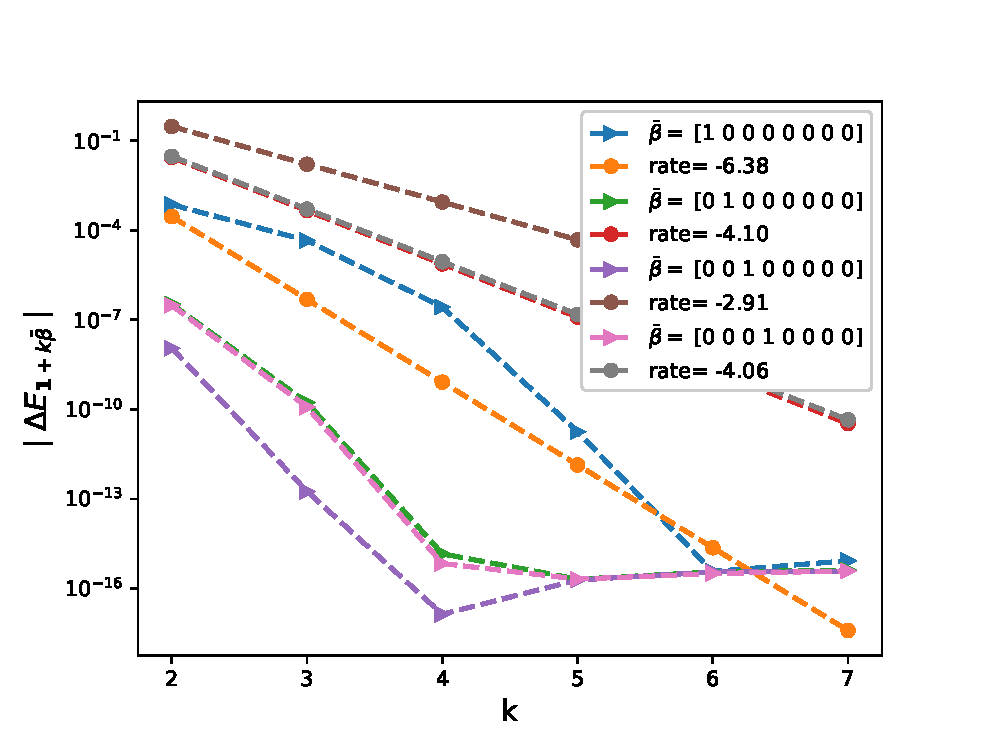
\includegraphics[width=1\linewidth]{./figures/rBergomi_mixed_error_rates/without_change_measure/N_4/H_002/first_difference_rbergomi_4steps_H_002_K_1_totally_hierarch_with_rate_W1}
		\caption{}
		\label{fig:sub3}
	\end{subfigure}%
	\begin{subfigure}{.4\textwidth}
		\centering
		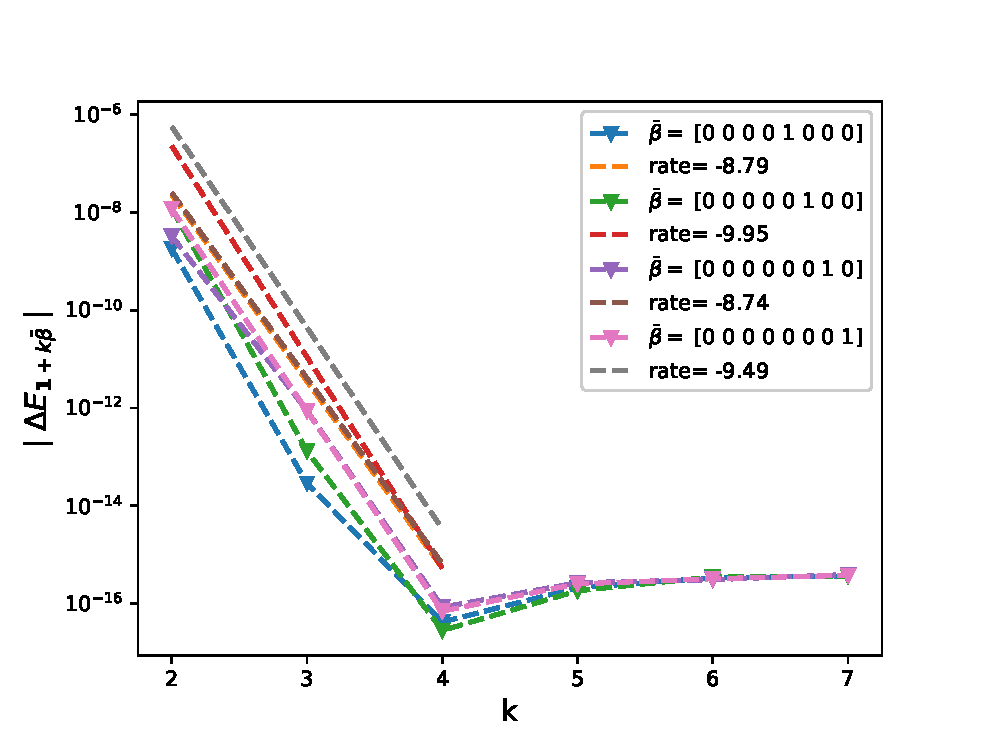
\includegraphics[width=1\linewidth]{./figures/rBergomi_mixed_error_rates/without_change_measure/N_4/H_002/first_difference_rbergomi_4steps_H_002_K_1_totally_hierarch_with_rate_W2}
		\caption{}
		\label{fig:sub4}
	\end{subfigure}
	
	
	
	\caption{The rate of error convergence of first order differences $\abs{\Delta \text{E}_{\boldsymbol{\beta}}}$ \eqref{eq:Work_error_contributions} ($\boldsymbol{\beta}=\mathbf{1}+k \bar{\boldsymbol{\beta}}$) with respect to $\mathbf{W}^{(1)}$ (a)  and  with respect to $\mathbf{W}^{(2)}$ (b), for parameter set $2$ in Table \ref{table:Reference solution, using MC with $500$ time steps, of Call option price under rBergomi model, for different parameter constellation.}. The number of quadrature points used in the $i$-th dimension is $N_i=2^{\beta_i-1}+1$. }
	\label{fig:first_diff_comp_K_1_H_002}
\end{figure}


\begin{figure}[h!]
	\centering
	\begin{subfigure}{.4\textwidth}
		\centering
		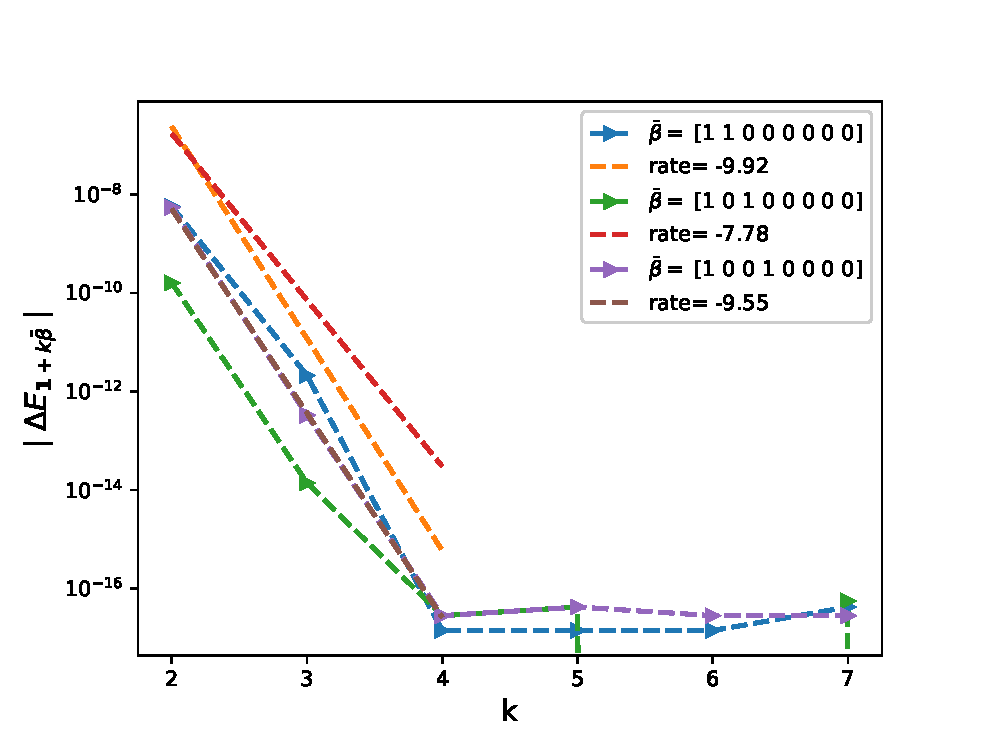
\includegraphics[width=1\linewidth]{./figures/rBergomi_mixed_error_rates/without_change_measure/N_4/H_002/mixed_difference_order2_rbergomi_4steps_H_002_K_1_totally_hierarch_with_rate_W1}
		\caption{}
		\label{fig:sub3}
	\end{subfigure}%
	\begin{subfigure}{.4\textwidth}
		\centering
		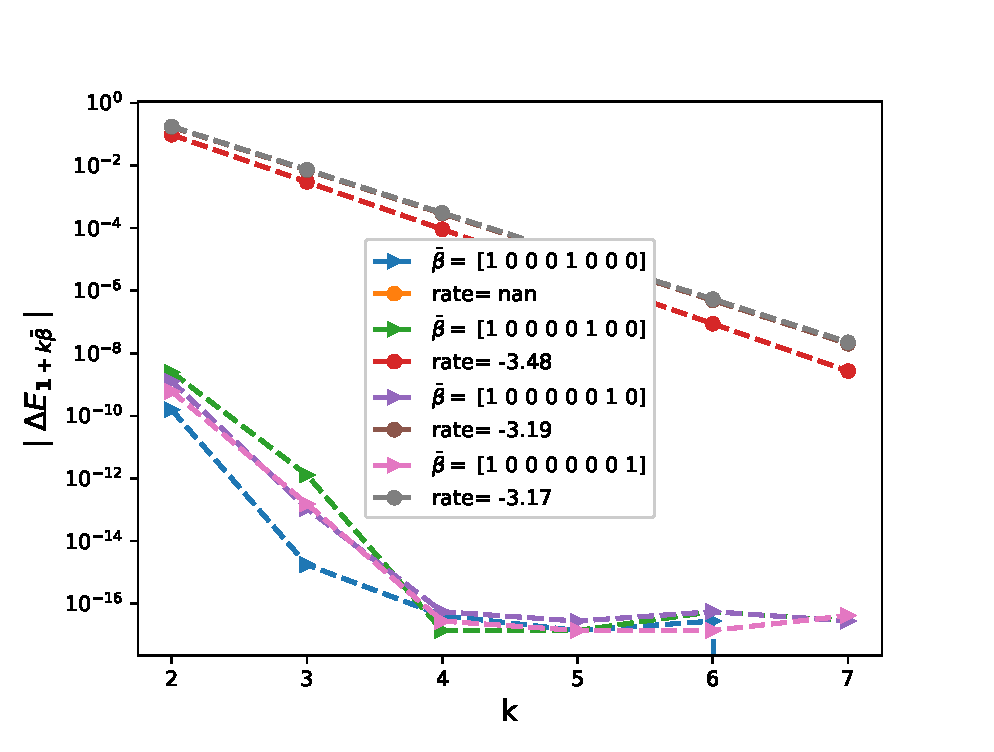
\includegraphics[width=1\linewidth]{./figures/rBergomi_mixed_error_rates/without_change_measure/N_4/H_002/mixed_difference_order2_rbergomi_4steps_H_002_K_1_totally_hierarch_with_rate_W2}
		\caption{}
		\label{fig:sub4}
	\end{subfigure}
	
	\caption{The rate of error convergence of  second order differences $\abs{\Delta \text{E}_{\boldsymbol{\beta}}}$ \eqref{eq:Work_error_contributions}  ($\boldsymbol{\beta}=\mathbf{1}+k \bar{\boldsymbol{\beta}}$) with respect to $\mathbf{W}^{(1)}$ (a)  and  with respect to $\mathbf{W}^{(2)}$ (b), for parameter set $2$ in Table \ref{table:Reference solution, using MC with $500$ time steps, of Call option price under rBergomi model, for different parameter constellation.}. The number of quadrature points used in the $i$-th dimension is $N_i=2^{\beta_i-1}+1$.}
	\label{fig:second_diff_comp_K_1_H_002}
\end{figure}

\FloatBarrier

%
%\begin{remark}
%	In this paper, we limited ourselves to designing a novel alternative method  based on hierarchical adaptive sparse grids quadrature for computing option prices under the rBergomi model. Giving the significant performance gains of our novel designed algorithm, we expect that designing a method based on QMC can bring similar or more gains as  our approach.
%\end{remark}



\subsection{Brownian bridge construction}\label{sec:Brwonian bridge construction}
In the literature of adaptive sparse grids and  QMC, several hierarchical path generation methods (PGMs) or transformation methods have been proposed to reduce the effective dimension. Among these transformations, we cite  the Brownian
bridge (Bb)  construction \cite{morokoff1994quasi,moskowitz1996smoothness,caflisch1997valuation}, the principal component analysis (PCA)  \cite{acworth1998comparison} and the linear transformation (LT) \cite{imai2004minimizing}.

In our context, the Brownian motion on a time discretization can be constructed either sequentially using a standard random walk construction or hierarchically using   other hierarchical PGMs as listed above. For our purposes, to make an effective use of MISC, which profits from anisotropy, we use the Bb construction since it produces  dimensions with different importance for MISC, contrary to random walk procedure for which all the dimensions of the stochastic space have equal importance.  This transformation  reduces the effective dimension  of the problem and as a consequence accelerates the MISC procedure by reducing the computational cost.


Let us denote $\{t_i\}_{i=0}^{N}$ the grid of time steps. Then the Bb construction \cite{glasserman2004monte} consists of the following: given a past value $B_{t_i}$ and a future value $B_{t_k}$, the value $B_{t_j}$ (with $t_i < t_j < t_k$) can be generated according to 
\begin{equation}
B_{t_j}=(1-\rho) B_{t_i}+\rho B_{t_k}+ \sqrt{\rho (1-\rho)(k-i) \Delta t} z, \: z \sim \mathcal{N}(0,1) \COMMA
\end{equation}
where $\rho=\frac{j-i}{k-i}$.  


%In particular, if $N$ is a power of $2$, then given $B_0=0$, Bb generates the Brownian motion at times $T, T/2,T/4,3T/4,\dots$ according
%\begin{align}\label{eq:BB construction}
%	B_T&=\sqrt{T}z_1\nonumber\\
%	B_{T/2}&= \frac{1}{2}(B_{0}+B_{T})+\sqrt{T/4}z_2= \frac{\sqrt{T}}{2} z_1+\frac{\sqrt{T}}{2} z_2\nonumber\\
%	B_{T/4}&=\frac{1}{2} (B_{0}+B_{T/2})+\sqrt{T/8}z_3= \frac{\sqrt{T}}{4} z_1+\frac{\sqrt{T}}{4} z_2+\sqrt{T/8}z_3\nonumber\\
%	\vdots \nonumber\\
%\end{align}
%where $\{z_j\}_{j=1}^{N}$ are independent standard normal variables.  In Bb construction scheme given by \eqref{eq:BB construction}, the most important values that determine the large scale structure of Brownian motion are the first components of $\mathbf{z} = (z_1,\dots,z_N)$.



%\begin{remark}
%In this paper, we chose to couple Brownian bridge construction with the MISC solver to reduce the effective dimension, since it is the less costly option in terms of computational work and the easiest to implement. We did not investigate the performance of MISC when coupling it with other hierarchical path generations method such as PCA or LT, which could be left as a future work that looks for the optimal PGM to couple with MISC in this context.
%\end{remark}
%


\subsection{Richardson extrapolation}\label{sec:Richardson extrapolation}


Another transformation that we coupled with MISC is Richardson extrapolation \cite{talay1990expansion}. In fact, applying level $K_\text{R}$ (level of extrapolation) of Richardson extrapolation reduces dramatically the bias and as a consequence reduces the  number of time steps $N$ needed in the coarsest level to achieve a certain error tolerance. This means basically that Richardson extrapolation directly reduces  the total dimension of the integration problem for achieving some error tolerance.


We  recall that the Euler scheme has weak order one so that

\begin{align}\label{Euler_weak_error}
	\abs{\expt{f(\hat{X}_T^h)}-\expt{f(X_T)} }  \leq C h
\end{align}

for some constant $C$, all sufficiently small $h$ and suitably smooth $f$. It can be easily  shown that  \eqref{Euler_weak_error} can be improved to


\begin{align}\label{Euler_weak_error_strenghten}
	\expt{f(\hat{X}_T^h)}= \expt{f(X_T)} + c h +\Ordo{h^2} \COMMA
\end{align}


where $c$ depends on $f$. 

Applying \eqref{Euler_weak_error_strenghten} with discretization step $2h$, we  obtain

\begin{align}\label{Euler_weak_error_strenghten_2h}
	\expt{f(\hat{X}_T^{2h})}= \expt{f(X_T)} + 2 c h +\Ordo{h^2} \COMMA
\end{align}

implying

\begin{align}\label{Richardson_extrapol}
	2 \expt{f(\hat{X}_T^{2h})}- \expt{f(\hat{X}_T^{h})} =\expt{f(X_T)} + \Ordo{h^2} \COMMA
\end{align}

For higher levels of extrapolations, we use the following: Let us denote by $h_J=h_0 2^{-J}$ the grid sizes (where $h_0$ is the coarsest grid size), by $K_\text{R}$ the level of the Richardson extrapolation, and by $I(J,K_\text{R})$ the approximation of $\expt{f((X_T)}$ by terms up to level $K_\text{R}$ (leading to a weak error of order $K_\text{R}$), then we have the following recursion 

\begin{align}
I(J,K_\text{R})=\frac{2^{K_\text{R}}\left[I(J,K_\text{R}-1)-I(J-1,K_\text{R}-1)\right]}{2^{K_\text{R}}-1},\quad J=1,2,\dots, K_\text{R}=1,2,\dots
\end{align}


\red{
\begin{remark}
We emphasize that through our work, we are interested in the pre-asymptotic regime (small number of time steps), and the use of Richardson extrapolation is justified by our observed experimental results in that regime (see Section \ref{sec:Weak error plots_no_change}),  which in, in particular, show an order one of convergence for the weak error. Although, we do not claim that the observed rates will scale well in the asymptotic regime, we observed that the pre-asymptotic regime is enough to get sufficiently accurate estimates for the option prices. 
\end{remark}
}



\section{ASGQ error estimate}\label{sec:MISC error estimate}
As discussed, potential ways of estimating the quadrature error are presented below.
\subsection{First way: Similar to the one implemented by Joakim}
I think this way is almost similar to the one implemented by Joakim. He may correct me if I missed some things.

In our case, once we fix $N$, we define from \eqref{BS_formula_rbergomi_2}
\begin{equation*}
F^N=C_{\text{BS}}(G(\mathbf{W}^{(1)},\mathbf{W}^{(2)})) \PERIOD
\end{equation*}
We introduce the set $C^0(\rset)$ of real-valued continuous functions over $\rset$, and the subspace of polynomials of degree at most $q$ over $\rset$, $\mathbb{P}^q(\rset) \subset C^0(\rset)$. Next,
we consider a sequence of univariate Lagrangian interpolant operators in each dimension $Y_n$ ($1 \le n \le 2N$), that is, $\{U_n^{m(\beta_n)}\}_{\beta_n \in \nset_+}$ (we refer to the value $\beta_n$ as the interpolation level). Each interpolant is built over a set of $m(\beta_n)$ collocation points, $\mathcal{H}^{m(\beta_n)}=\{y^1_n,y^2_n,\dots,y^{m(\beta_n)}_n\} \subset \rset$, thus, the interpolant yields a polynomial approximation,
\begin{equation*}
U^{m(\beta_n)}:C^0(\rset) \rightarrow \mathbb{P}^{m(\beta_n)-1}(\rset), \quad U^{m(\beta_n)}[F^N](y_n)= \sum_{j=1}^{m(\beta_n)} \left( f(y^j_n) \prod_{k=1;k \neq j}^{m(\beta_n)} \frac{y_n-y_n^k}{y_n^j-y_n^k}\right) \PERIOD
\end{equation*}
The $2N$-variate Lagrangian interpolant can then be built by a tensorization of univariate interpolants: denote by $C^0(\rset^{2N})$ the space of real-valued $2N$-variate continuous functions over $\rset^{2N}$ and by $\mathbb{P}^{\mathbf{q}}(\rset^{2N}) = \otimes_{n=1}^{2N} \mathbb{P}^{\mathbf{q}_n}(\rset)$ the subspace of polynomials of degree at most $q_n$ over $\rset$, with $\mathbf{q}=(q_1,\dots,q_{2N})\in  \nset^{2N}$, and consider a multi-index $\boldsymbol{\beta} \in \nset^{2N}_+$ assigning the interpolation level in each direction, $y_n$, then  the multivariate interpolant can then be written as
$$U^{m(\boldsymbol{\beta})}: C^0(\rset^{2N}) \rightarrow \mathbb{P}^{m(\boldsymbol{\beta})-1}(\rset^{2N}) ,\quad  U^{m(\boldsymbol{\beta})}[F^N](\mathbf{y})= \bigotimes_{n = 1}^{2N} U^{m(\beta_n)} [F^N](\mathbf{y}) \PERIOD $$
Given this construction, we can define the ASGQ interpolant  for approximating $F^N$, using a set of multi indices $\mathcal{I} \in \nset^{2N}$ as
\begin{equation}
I^{\mathcal{I}}[F^N]= \sum_{\boldsymbol{\beta} \in \mathcal{I}} \Delta U_N^{\boldsymbol{\beta}} \COMMA
\end{equation}
where 
\begin{equation*}
\Delta_i U_N^{\boldsymbol{\beta}} = \left\{ 
\aligned 
 U_N^{\boldsymbol{\beta}} &- U_N^{\boldsymbol{\beta}'}  \text{, with } \boldsymbol{\beta}' =\boldsymbol{\beta} - e_i, \text{ if } \boldsymbol{\beta}_i>0 \\
 U_N^{\boldsymbol{\beta}} &, \quad  \text{ otherwise,}
\endaligned
\right.
\end{equation*}
where $e_i$ denotes the $i$th $2N$-dimensional unit vector. Then, $\Delta
U_N^{\boldsymbol{\beta}}$ is defined as
\begin{equation*}
\Delta U_N^{\boldsymbol{\beta}} = \left( \prod_{i=1}^{2N} \Delta_i \right) U_N^{\boldsymbol{\beta}}.
\end{equation*}
We define the interpolation error induced by ASGQ as
\begin{equation}
e_{N}= F^N-I^{\mathcal{I}}[F^N] \PERIOD
\end{equation}
One can have a bound on the interpolation error of ASGQ, $e_{N}$, by tensorizing one dimensional error estimates, and  then simply integrate that bound to get the ASGQ  error, $\mathcal{E}_Q(\text{TOL}_{\text{ASGQ}},N)$, defined in \eqref{eq:total_error_ASGQ}. However, we think that this will  not lead to a sharp error estimate for ASGQ. Another strategy for estimating the ASGQ  error, is to estimate $\expt{e_N}$ using MC by sampling directly $e_N$ (what I think Jaokim code is doing actually) .

If we define $Y=F^N+(Q_N^{\mathcal{I}}-I^{\mathcal{I}}[F^N])$ (where $Q_N^{\mathcal{I}}$ is the ASGQ  estimator), then we have
\begin{align}\label{eq:Control_variate}
\expt{Y}&=\expt{F^N}\nonumber\\
Var[Y]&=Var[e_N]< Var[\mathcal{A}_{\text{MC}}]\COMMA
\end{align}
where $\mathcal{A}_{\text{MC}}$ is the MC estimator for $\expt{F^N}$.

\eqref{eq:Control_variate} shows that ASGQ can be seen as a control variate for MC estimator and consequently as a powerful variance reduction tool.

This way of estimating the quadrature error comes with the disadvantage of exciting the strong error which has a poor behavior in our context resulting maybe to having a non-sharp error estimate. In fact, by the central limit theorem, we expect that
\begin{align}\label{eq:CLT_interpol_errror}
\abs{\expt{e_N}}&=\abs{\int \underbrace{F^N-I^{\mathcal{I}}[F^N](y)}_{Y(y)} dy}\nonumber\\
&\approx \frac{C_\alpha}{\sqrt{M}} \sqrt{\text{Var(Y)}}\PERIOD
\end{align}
In our context of the rBergomi model we know that the strong error is of order $H$, that is we expect to have $\text{Var(Y)}=\Ordo{h^H}$ ($h$ is the mesh size and $H$ is the Hurst parameter which is of order $\approx 0.1$. As a consequence, it may be that using this way will not provide a sharp enough error estimate for the quadrature error!

\subsection{Second way}
To avoid exciting the strong error when estimating the quadrature error and just act on the weak error, we can use a second way that is inspired of randomized QMC. In fact, we suggest to use a randomized version of ASGQ where the randomization involves randomized rotation and scaling for quadrature rules since we deal with unbounded domains and Hermite quadrature rule. Although this comes with the advantage of just acting on the weak error, it has the issue of reducing anisotropy which is a main feature for a good performance of ASGQ.

We can formulate this more in case the first way fail!

\subsection{Third way}
One can learn the error curve as a way to reduce the extra burden that comes
from estimating the ASGQ error but this not yet formulated yet. I will try to formulate it if the two previous options fail!

\section{Numerical experiments of estimating quadrature error}\label{sec:Numerical tests}
In this section, I show the obtained quadrature estimates for one of my examples for $N=2,4,8$ where $N$ is the number of time steps.  Looking at Figure \ref{fig:Quadrature and interpolation error estimation for 3 different cases of number of time steps}, I have some questions  that are not clear to me:
\begin{itemize}
\item $\mathbf{Q}_1$: I did not get why the quadrature error is kind of constant and then it decays so fast for very large number of collocation points. Is it normal to observe such behavior? Also, this behavior is less weird when taking $N=8$.

 $\mathbf{A}_1$: This behavior as per Raul is not weird so It maybe that with few points we already rich an accuracy that remains constant ans as we have larger number of quadrature points we see this sharp decay, meaning the accuracy changes a lot for high number of quadrature points!

\item  $\mathbf{Q}_2$: Why the interpolation error seems to be constant?

 $\mathbf{A}_2$: This maybe due to the fact that the statistical error is already dominating the bias  as explained by \eqref{eq:CLT_interpol_errror}! so we do not see what really happens for the bias term

\item Does it seem that using the interpolation error as a bound for the quadrature error is not that good?
\end{itemize}

\begin{figure}
	\centering % <-- added
	\begin{subfigure}{0.6\textwidth}
		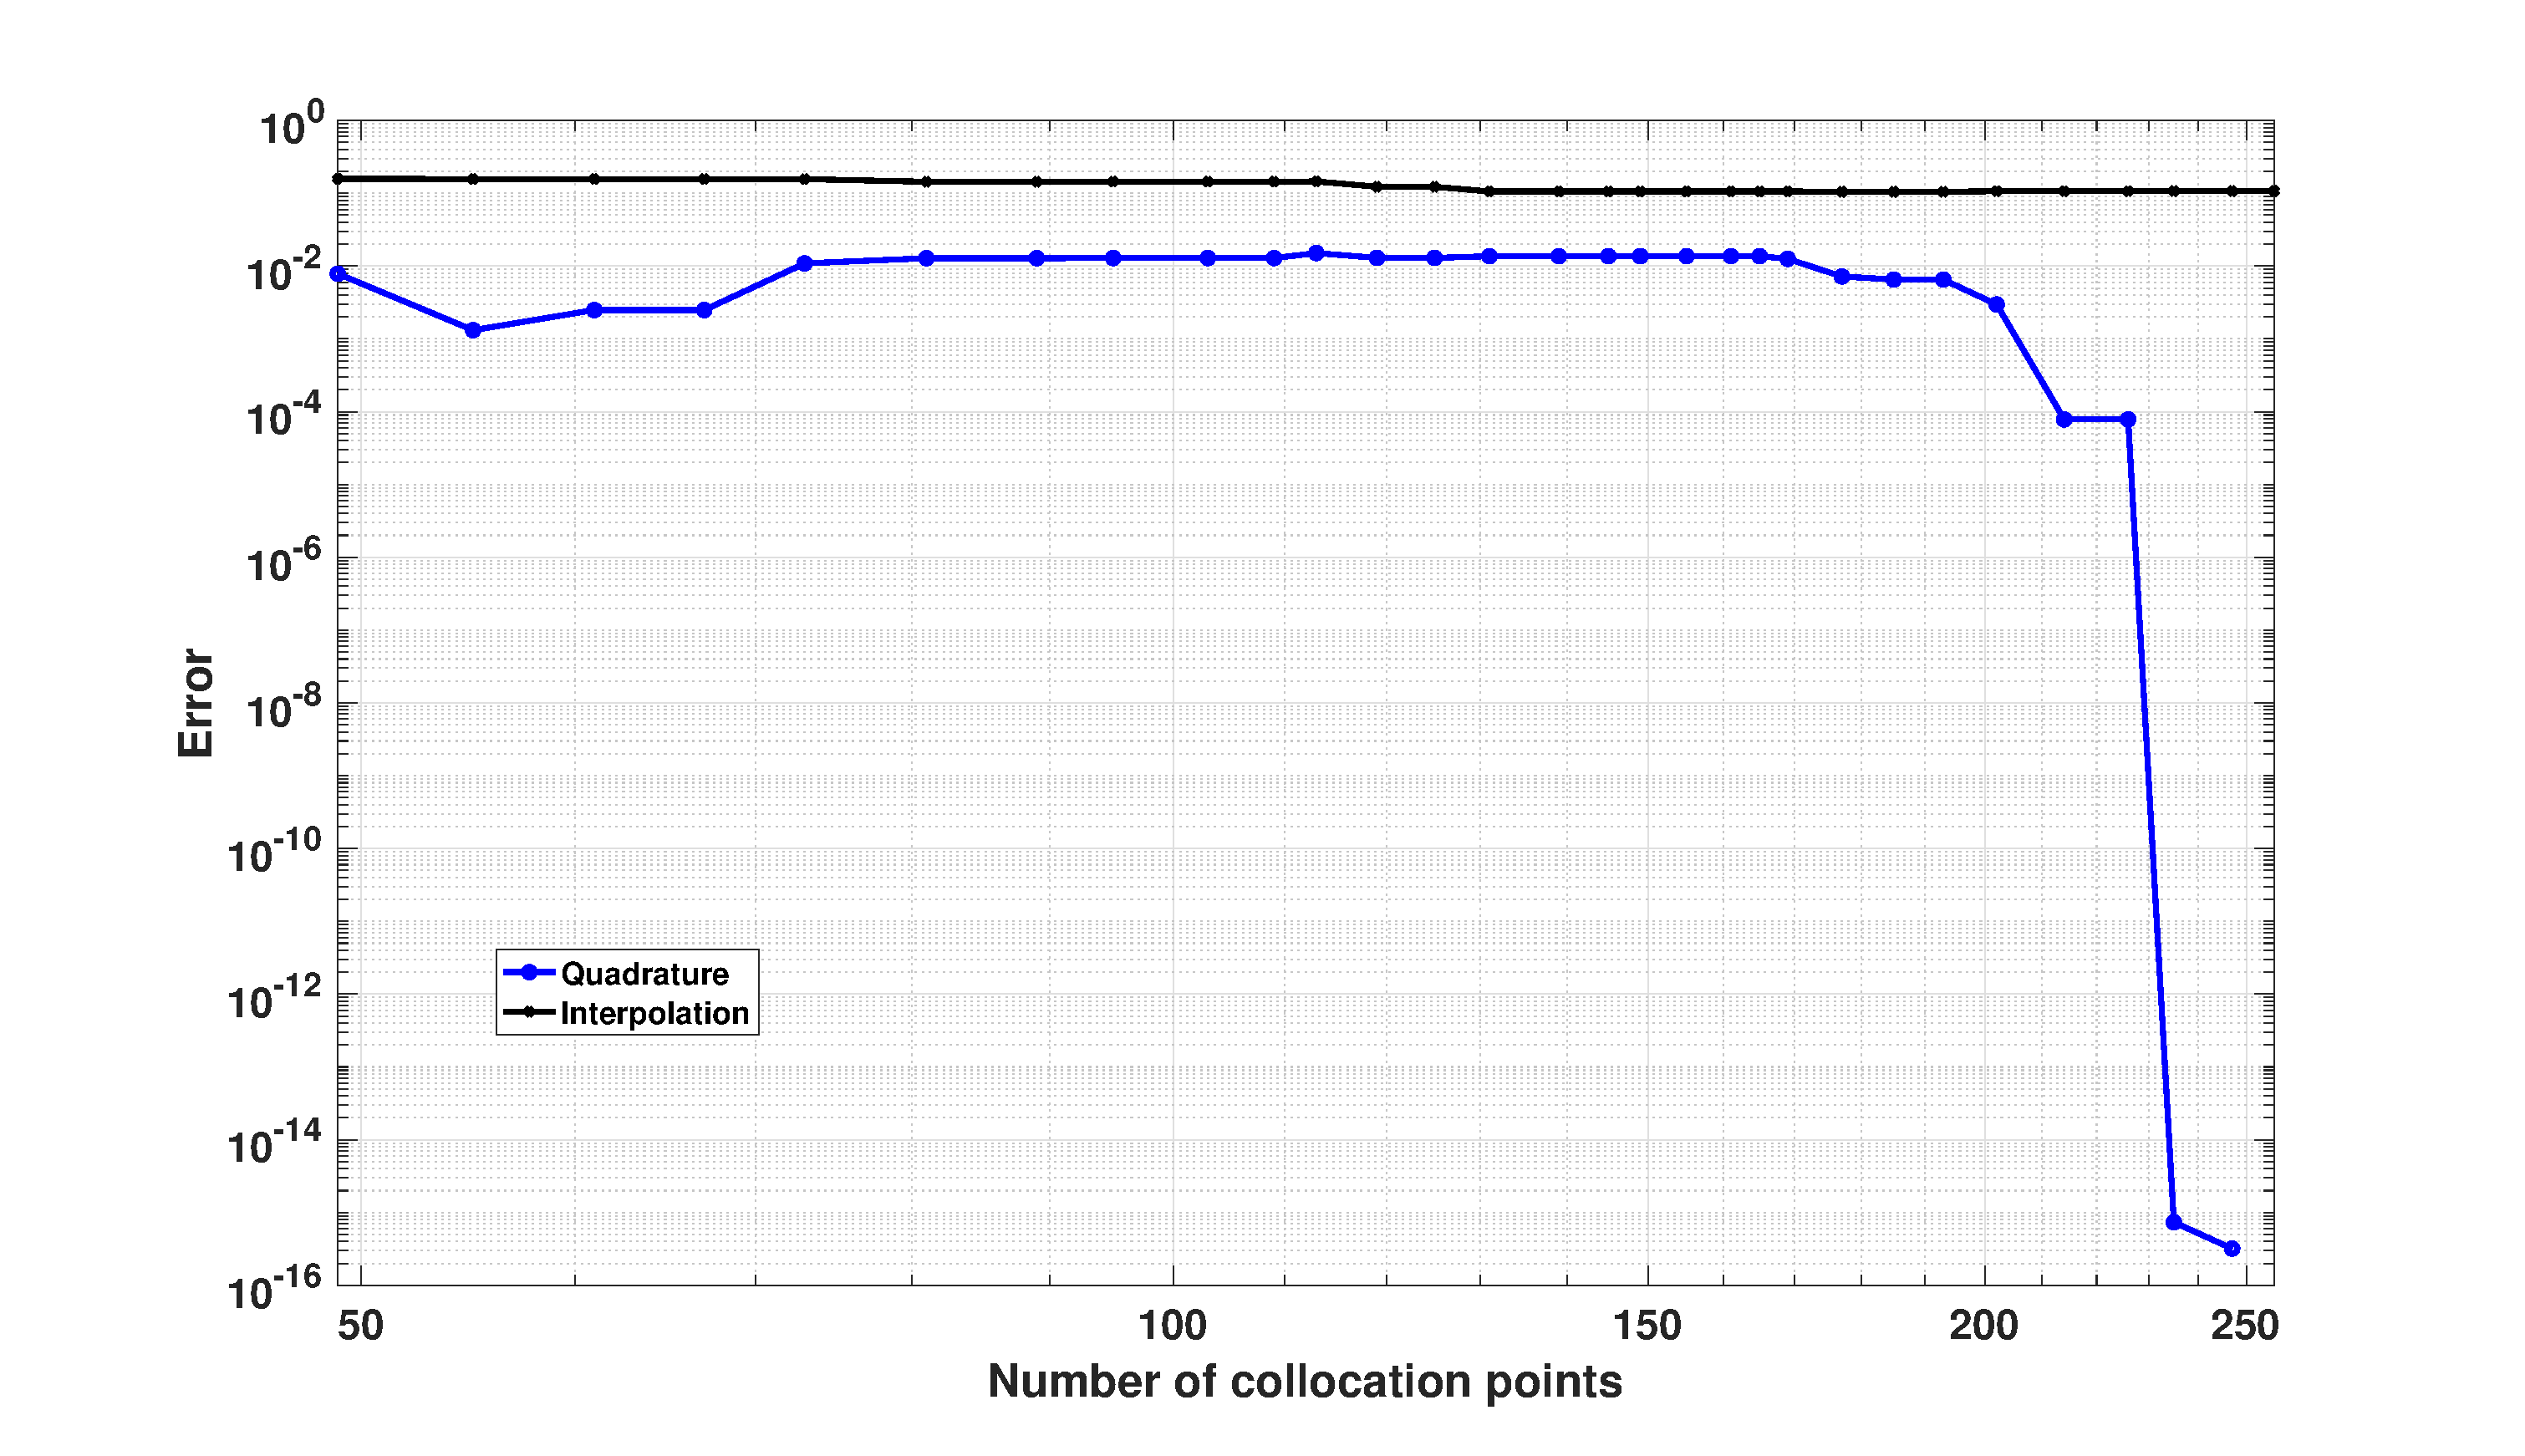
\includegraphics[width=\linewidth]{./case_N_2.eps}
		\caption{}
		\label{fig:1}
	\end{subfigure}\hfil % <-- added
	\begin{subfigure}{0.6\textwidth}
		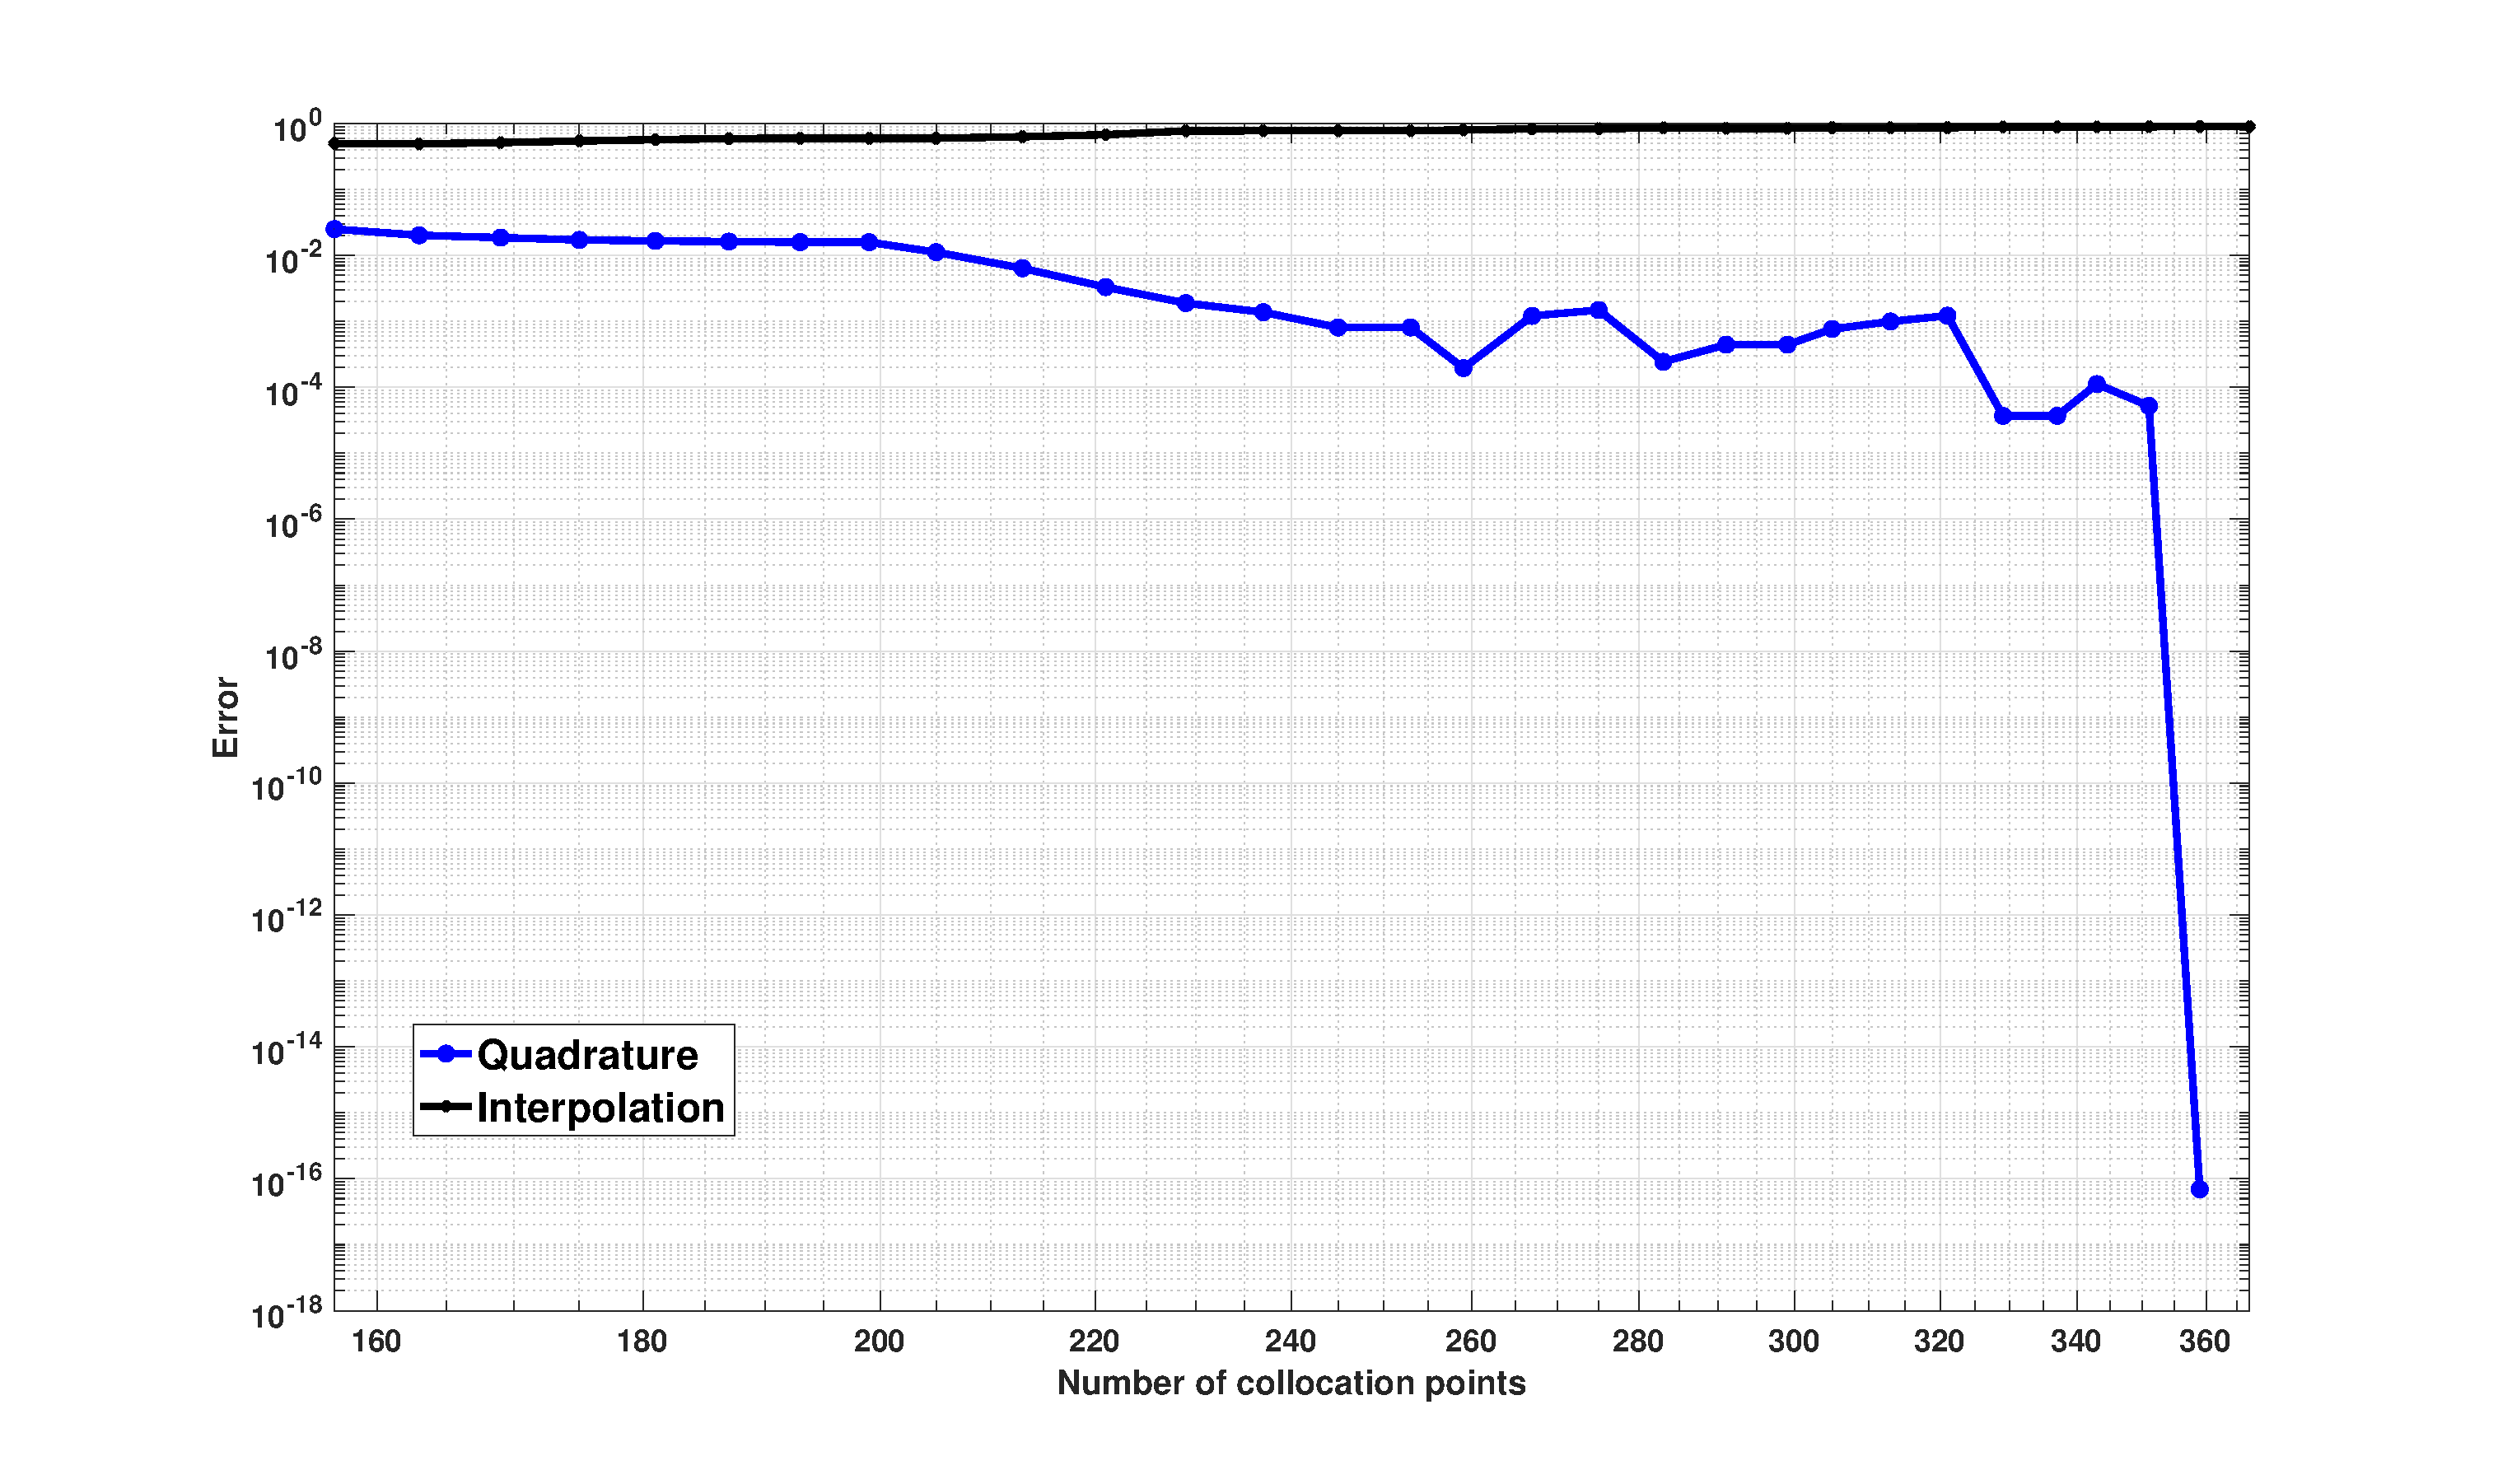
\includegraphics[width=\linewidth]{./case_N_4.eps}
		\caption{}
		\label{fig:2}
	\end{subfigure}\hfil % <-- added
	\begin{subfigure}{0.6\textwidth}
		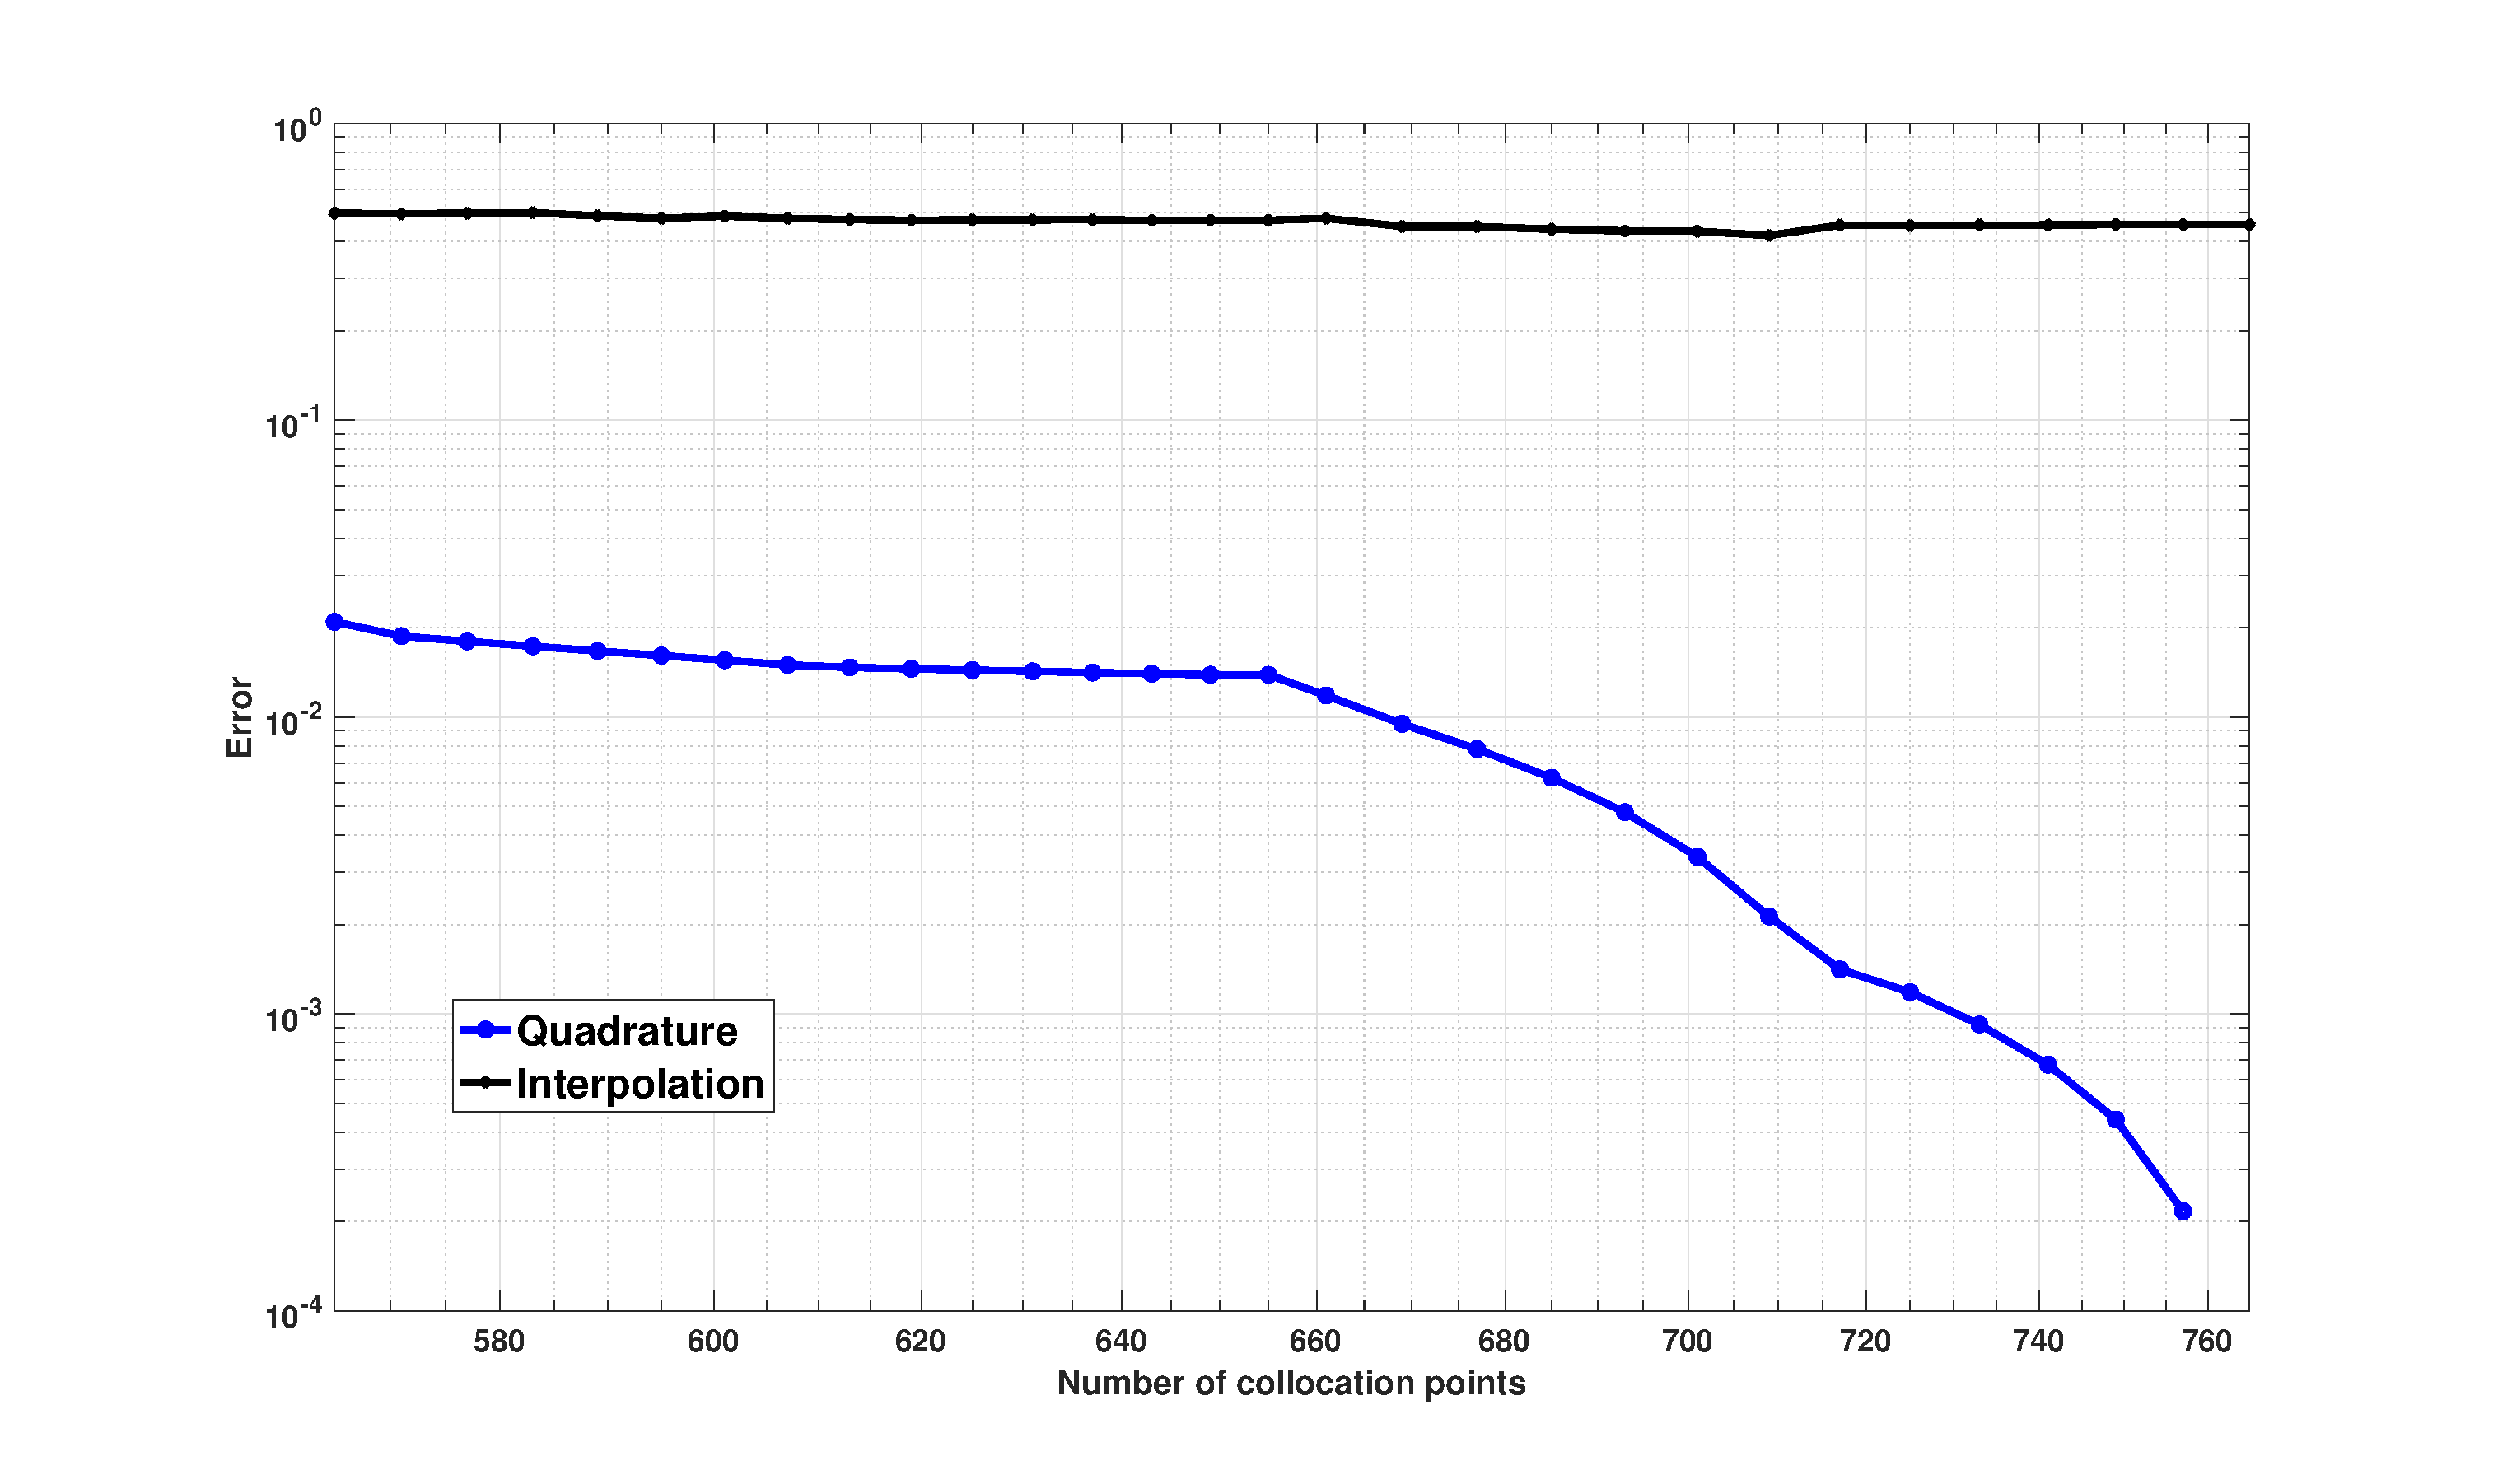
\includegraphics[width=\linewidth]{./case_N_8.eps}
		\caption{}
		\label{fig:3}
	\end{subfigure}
	\caption{Quadrature (computed as the difference between the quadrature solution and a reference solution computed with very high number of quadrature points),   and interpolation error  (as explained in the first way of Section \ref{sec:MISC error estimate}) for $3$ different cases of number of time steps: a) $N=2$, b) $N=4$,  c) $N=8$}
	\label{fig:Quadrature and interpolation error estimation for 3 different cases of number of time steps}
\end{figure}
\FloatBarrier



 %%%%%%%%%%%%%%%%%%%%%%%%%%%%%%%%%%%%%%%%%%
%References
%%%%%%%%%%%%%%%%%%%%%%%%%%%%%%%%%%%%%%%%%%

\bibliographystyle{plain}
\bibliography{smoothing_rBergomi.bib} 








 

 

 
 
 


\end{document}